% This is ``sig-alternate.tex" V1.8 June 2007
% This file should be compiled with V2.3 of ``sig-alternate.cls" June 2007
%
% This example file demonstrates the use of the 'sig-alternate.cls'
% V2.3 LaTeX2e document class file. It is for those submitting
% articles to ACM Conference Proceedings WHO DO NOT WISH TO
% STRICTLY ADHERE TO THE SIGS (PUBS-BOARD-ENDORSED) STYLE.
% The 'sig-alternate.cls' file will produce a similar-looking,
% albeit, 'tighter' paper resulting in, invariably, fewer pages.
%
% ----------------------------------------------------------------------------------------------------------------
% This .tex file (and associated .cls V2.3) produces:
%       1) The Permission Statement
%       2) The Conference (location) Info information
%       3) The Copyright Line with ACM data
%       4) NO page numbers
%
% as against the acm_proc_article-sp.cls file which
% DOES NOT produce 1) thru' 3) above.
%
% Using 'sig-alternate.cls' you have control, however, from within
% the source .tex file, over both the CopyrightYear
% (defaulted to 200X) and the ACM Copyright Data
% (defaulted to X-XXXXX-XX-X/XX/XX).
% e.g.
% \CopyrightYear{2007} will cause 2007 to appear in the copyright line.
% \crdata{0-12345-67-8/90/12} will cause 0-12345-67-8/90/12 to appear in the copyright line.
%
% ---------------------------------------------------------------------------------------------------------------
% This .tex source is an example which *does* use
% the .bib file (from which the .bbl file % is produced).
% REMEMBER HOWEVER: After having produced the .bbl file,
% and prior to final submission, you *NEED* to 'insert'
% your .bbl file into your source .tex file so as to provide
% ONE 'self-contained' source file.
%
% ================= IF YOU HAVE QUESTIONS =======================
% Questions regarding the SIGS styles, SIGS policies and
% procedures, Conferences etc. should be sent to
% Adrienne Griscti (griscti@acm.org)
%
% Technical questions _only_ to
% Gerald Murray (murray@acm.org)
% ===============================================================
%
% For tracking purposes - this is V1.8 - June 2007

\documentclass{sig-alternate}

\usepackage{epsfig}
\usepackage{cite}
\usepackage{verbatim}
\usepackage{graphicx}
\begin{document}

\title{Programming Environments for Mobile Ad Hoc Networks}

\begin{comment}
\conferenceinfo{WICON '08}{November 17-19, 2008, Maui, Hawaii, USA}
%\CopyrightYear{2007} % Allows default copyright year (200X) to be over-ridden - IF NEED BE.
%\crdata{0-12345-67-8/90/01}  % Allows default copyright data (0-89791-88-6/97/05) to be over-ridden - IF NEED BE.
% --- End of Author Metadata ---
\end{comment}

\title{Programming Environments for Mobile Ad Hoc Networks}
%\subtitle{[Extended Abstract]

\numberofauthors{2} 
\author{
% 1st. author
\alignauthor
Justin Collins\\
       \affaddr{Mobile Systems Lab}\\
       \affaddr{Computer Science Department}\\
       \affaddr{University of California, Los Angeles}\\
       \affaddr{Los Angeles, California 90095}\\
       \email{collins@cs.ucla.edu}
% 2nd. author
\alignauthor
Rajive Bagrodia\\
       \affaddr{Mobile Systems Lab}\\
       \affaddr{Computer Science Department}\\
       \affaddr{University of California, Los Angeles}\\
       \affaddr{Los Angeles, California 90095}\\
       \email{rajive@cs.ucla.edu}
}


\maketitle
\begin{abstract}
The possibility for spontaneous ad hoc networks between mobile devices has been increasing as small devices become more capable of hosting useful networked applications. These applications face the challenges of frequenct disconnections, highly dynamic network topologies, and varying communication patterns, a combination unique to mobile ad hoc networks. This is the first survey to examine current MANET programming approaches including tuple spaces, remote objects, publish/subscribe, and code migration through analysis and experimental results. These approaches are essentially extensions to existing distributed and parallel computing concepts. We suggest that new abstractions may be necessary to fully handle the programming issues presented by MANETS.

\end{abstract}

\section{Introduction}

Mobile ad hoc networks (MANET) composed of small, portable devices are becoming more and more common. Many PDAs, smartphones, portable gaming systems and nearly all laptop computers now come equipped with the capability to form wireless ad hoc networks. Mobile applications are no longer limited to stand-alone or client-server programs, but can interact and form useful networks directly with each other. Such networks are ideal for situations in which there is no time to set up a fixed access point, or when there is no fixed infrastructure available. 


The ad hoc nature of these networks, combined with the mobility of the nodes, introduces new challenges. Dynamically formed groups of mobile nodes must be able to coordinate between themselves to perform routing and resource discovery. Routes between nodes and available resources may change rapidly, requiring flexible protocols. Nodes cannot rely on knowing the addresses of remote resources ahead of time or on a central directory, but must dynamically discover resources. Disconnections due to mobility and wireless channel variations become commonplace rather than exceptional.

Many new applications, particularly in the consumer space, are being applied to MANETs. These include disaster recovery scenarios, collaborative software such as shared whiteboards, impromptu networks for communication and entertainment, and peer-to-peer applications for file sharing. Much work has been done on protocol development for MANETs, such as AODV~\cite{aodv} and OLSR~\cite{olsr}, but systems supporting development of applications which can be used in a MANET are an active area of research. Currently, techniques which address issues specific to MANETs need to be tediously re-implemented in each application.

This paper focuses on the approaches used in recent and ongoing projects which provide environments in which to develop generic applications for the general case of MANET, which is completely infrastructureless with highly mobile wireless devices. Section 2 provides an overview of the requirements and issues specific to developing applications to run on MANETs. Section 3 is an overview of several projects which have been proposed and developed to meet those requirements, while Section 4 discusses the various solutions used by the projects in more detail. In Section 5, we attempt to gain a better understanding of techniques required for MANET application development by writing two sample applications using three different projects. Experimental evaluation of those three projects are presented in Section 6. Section 7 discusses related projects and Section 8 presents our conclusions.

\section{MANET Requirements}

Mobile applications face several challenges when compared with programs intended for standard desktops. Mobile devices are generally constrained in many ways: the screen size, processor power, memory, and battery power are often limited. Development platforms for mobile devices can provide basic libraries for application support such as menus and access to data stored on the device. Networking, however, is generally limited to sockets, TCP/IP, and HTTP. In particular, applications are expected to either stand-alone, like a calculator, or to only be using the network in a client-server manner, such as accessing websites or email servers.

However, the distinguishing characteristic of a MANET context is not the mobile device itself,  but the communication between devices. The primary medium for communication is wireless with no fixed infrastructure and nodes which tend to be highly mobile. In such an environment, the following become important requirements when developing applications:

\textit{Disconnection handling:} In a MANET, nodes are highly mobile and disconnections occur frequently, either due to channel condition variation or the mobility of end nodes and intermediate nodes. Disconnections may be prolonged, brief, or intermittent and applications must handle all three. Traditional networking treats disconnections as failures, but a programming environment for MANETs needs to handle disconnections as a natural element of the environment.

\textit{Addressing and discovery:} The lack of infrastructure in a MANET requires a decentralized method for finding and addressing resources. Traditional approaches such as DNS cannot be maintained in a MANET, so alternative means of discovering and addressing resources must be provided. The spontaneous nature of MANETs also dictates that discovery be dynamic, as the network topology cannot be known ahead of time and can change rapidly.

\textit{Flexible communication:} Both unicast and multicast communications are common in MANET applications, which are often group-based or collaborative. Being able to provide flexible communication is crucial to developing applications for MANETs.

\section{Project Overviews}

The current projects for developing software in MANETs fall into three broad categories: runtimes, languages, and middleware, which offer increasing levels of abstraction for the developer. They can also be combined: a middleware solution can be written in a language which uses one of the basic runtimes for mobile devices. In many cases projects also provide additional resources for software development such as debuggers and emulators for testing code. Table 1 summarizes the projects discussed in this paper with respect to the requirements in Section 1. A broader overview focusing only on middleware for MANETs can be found in~\cite{middlewaresurvey}.

\begin{table*}
\centering
\caption{Projects Summary}
\begin{tabular}{|c|c|c|c|c|c|} \hline
Project & Category & Disconnection Handling & Addressing and Discovery & Communication \\ \hline
LIME & Middleware & Tuple removal & Merged tuple spaces & Tuple space \\ \hline
MESHMdl & Middleware & Tuple removal & Tuple exchange & Tuple space \\ \hline
TOTA & Middleware & Connectionless & Tuple propagation & Tuple space \\ \hline
STEAM & Middleware  & Connectionless & Event content & Publish/subscribe \\ \hline
SyD & Middleware &  Object proxies &  Object type & Message passing \\ \hline
M2MI & Language & Connectionless &  Object type & Message passing \\ \hline
AmbientTalk & Language &  Flexible references &  Object type & Message passing \\ \hline
\begin{comment}YCab & Middleware &  State recovery &  Sessions, handles & Message passing \\ \hline\end{comment}
SpatialViews & Language & Connectionless & Object type & Code migration \\ \hline
.NET CF & Runtime &  None & URL & Sockets \\ \hline
Java ME & Runtime & None & URL & Sockets \\ \hline
\end{tabular}
\end{table*}

\subsection{Runtimes}

Runtimes in this context are virtual machines for languages which are specifically intended for use on small, resource-constrained mobile devices. Runtimes are useful because they provide good portability for applications and thereby simplify some of the application development process.

Two common runtimes for mobile devices are Java ME~\cite{javame} and the .NET Compact Framework~\cite{dotnetcf}. A third runtime, BREW~\cite{brew}, is a proprietary product from Qualcomm. These runtimes focus on using few resources and providing libraries for application development, especially user interfaces. They do not provide much networking support beyond basic sockets and HTTP support. While it is possible to use these runtimes as foundations for better abstractions, they provide little on their own to support MANET applications and will not be considered in the following comparisons.

\subsection{Languages}

A language in this paper refers to any language, language extension, or library which provides new language constructs for programming in a MANET. Languages often include their own runtime or are built on top of existing runtimes. Libraries and language extensions are likely to be easier for developers to use if they are already familiar with the base language.

M2MI~\cite{m2mi}, AmbientTalk~\cite{at1}, and SpatialViews~\cite{nisv} are three language-based projects intended for MANETs. Many-to-Many Invocation (M2MI) avoids costly ad hoc routing and discovery by broadcasting messages. Messages are addressed by object type, so if a device hosts an object of the addressed type, it will pass the message to that object.

The advantage of M2MI is simplicity. As messages are simply broadcast without expectation of reply, there is no need to worry about return values or blocking while waiting for confirmation. At the language level, there is no difference on the sender's side between a message which is actually received and one which is not received by anyone. Though this provides simplicity, it also means more work for the programmer. As there is no guarantee of message delivery, any functionality beyond simple unidirectionaly message passing must be implemented on top of M2MI.


AmbientTalk is a complete object oriented language inspired in part by M2MI's message passing. AmbientTalk implements a higher level abstraction of resource discovery and disconnection handling which is absent from M2MI, but retains the idea of object handles and remote method invocations. All remote events are handled asynchronously by AmbientTalk through the registration of callbacks. A block of code may be registered to be invoked when discovering a certain resource type. AmbientTalk also adds the ability to receive values from method invocations on remote objects through the use of futures. By default, messages sent to remote objects are buffered until they can be sent. The programmer can also choose to break the connection and recall buffered messages.


SpatialViews takes a completely different approach than M2MI and AmbientTalk. SpatialViews is a language extension to Java ME which allows programs to iterate over groups of devices. The code inside the loop is executed on the initial device and then migrates to the next, eventually making its way back to the initial node. This allows for complex operations to be written easily, as the language has built-in support for such things actions as reduction operations. The iteration itself is generally done according to some physical layout, although it is possible to iterate over all objects or to use logical locations instead.

\subsection{Middleware}

Middleware is software which manages interaction and communication between applications, as well as providing various services which may be used by applications. Middleware may also include supporting libraries which can be used by applications.

LIME (Linda in mobile environment)~\cite{lime} is a well-established implementation of tuple spaces\cite{linda} for mobile environments. Each device or agent has its own tuple space, which can merge with remote tuple spaces when they come into range of each other. Tuples can be read and written from specific locations, but can also be read or written to the ``federated" tuple space which includes the local tuple space and any tuple spaces which are currently merged with it. However, the tuple will reside in a particular tuple space, so when that device or agent moves away, the tuples in that tuple space will move with it and be out of reach. LIME does not currently have an implementation intended for mobile devices smaller than laptops, though there are variations of LIME intended for sensors.

MESH\textit{Mdl}~\cite{meshmdl}  is another tuple space implementation, but varies slightly from the LIME model. In MeshMdl, there is a single tuple space shared between all applications on a device. All communication between applications is done through this shared tuple space. Remote tuple spaces are not shared like in LIME, but are accessible for reads and writes only: it is not possible to remove tuples from a remote tuple space. MESH\textit{Mdl} supports mobile agents and recommends using them if actions need to be performed on a remote tuple space. MESH\textit{Mdl} also adds the idea of being able to automatically write, read, or block tuples from other tuple spaces.

Tuples on the Air (TOTA)~\cite{tota}  also implements a tuple space for MANETs, but differs from LIME and MESH\textit{Mdl}. Rather than storing tuples on a particular device, tuples in TOTA are propagated through the network according to rules specified per tuple. As the tuples move through the network, they can acquire context information about the network, such as how many hops they have traveled from the source.

SyD (System on Mobile Devices)~\cite{syd} is a complete middleware solution for MANETs. The middleware centers around the idea of object registries which allows service registration and lookup. Methods can then be invoked on these remote objects. Disconnection is handled by allowing objects to also provide proxy objects. If an object is unavailable, the method invocation will be handled by the proxy object, which can then perform an action specific to that service. For example, the proxy may buffer the request and send it later, or send back a cached or default response.

STEAM (Scalable Timed Events and Mobility)~\cite{steam} is an event-driven middleware which uses a publish/subscribe\cite{pubsubsurvey} mechanism for propagating events. STEAM uses the concept of proximity groups for communication, limiting events to the local geographic area. Events are propagated by subscribers only when the subject and proximity match. Events are further filtered on the subscriber side by content, which determines if an event is delivered to the local application.

\section{Approaches to Requirements}

\subsection{Disconnection Handling}

The main challenge in MANETs is handling disconnections, which may be intermittent, prolonged, or permanent. For example, at a busy conference there may be many mobile devices in contact with each other, but distance and physical obstacles may cause intermittent disconnections. Routes may also break and reform due to mobility or channel variations, possibly causing prolonged disconnections, but connections are eventually regained. When the attendees all leave, it becomes unlikely their devices will ever be in contact with each other again, making the disconnection permanent. A programming environment for MANETs must be able to handle all three kinds of disconnections.

One solution, used in LIME, MESH\textit{Mdl}, and TOTA, is to use tuple spaces for communication. Tuple spaces exhibit both spatial and temporal decoupling, meaning that messages being sent do not need to be addressed to a particular recipient nor does the recipient need to be present when the message is sent. Tuple spaces generally operate by reading, writing, and taking tuples to and from a shared location. Rather than sending a message directly to a recipient, a tuple is written to the tuple space and can be read or taken from the tuple space by other clients. This allows the tuple space to withstand disconnections.

For example, a tuple may be written out to the tuple space and then retrieved by a different client an arbitrary amount of time later. The client which retrieves the tuple may not even be in existence when the tuple was written. However, there is still a problem if the writer of the tuple disconnects before the tuple is read by a receiver. For LIME and MESH\textit{Mdl}, where the tuple space is associated with a particular devices, the tuple space is only available when the sender and the receiver are able to communicate directly with each other. In TOTA, tuples are disseminated throughout the network and can survive even if the original sender disconnects.

A different approach, used by M2MI and STEAM, is to forgo connections completely. Messages in M2MI are sent with no expectation of reply. In the general case, messages are sent to a particular object type, to be processed by any device hosting an object of that type. Messages are broadcast with no bufbroadcast with no bufferingwhether or not there is a receiver available. This provides even more decoupling than tuple spaces, but tuple spaces have the advantage of having some feedback about a tuple's status. The sender can check if a tuple has been removed from the tuple space or not. If it has, the sender can have some assurance the tuple was received by someone, otherwise it will be available until removed by the original sender or another client.

STEAM avoids connections by filtering events on the subscriber's side. This eliminates the need for publishers to keep track of subscribers and completely decouples the two. However, publish/subscribe in a MANET environment does not provide any message reliability. Any message reliability or disconnection feedback would need to be implemented on top of the publish/subscribe framework.

Code migration, the approach used by SpatialViews, does not maintain connections, but can be affected by disconnections if the device currently executing the mobile code fails or leaves the network before completion.  Most of the devices in the network will not be involved in executing code at any particular moment, in which case their failure or disconnection from the network would not have an effect. When it does have an effect, however, it may cause the entire iteration to fail. This can be mitigated by using a form of parallel iteration over the devices. Since the iteration order in SpatialViews is nondeterministic, it does not provide message reliability.

A third approach, implemented in AmbientTalk, relies on event handling and futures. Event handlers can be registered for various events, such as discovery of a service or disconnection of a remote object. Figure~\ref{fig:atpd} illustrates the use of two of these callbacks to discover a printer service. Once a printer is discovered, a document is sent to be printed and a status message is returned.  If a remote object is discovered and later moves out of range, AmbientTalk can call the disconnection code. By default, messages sent to a disconnected remote object will be buffered until it is possible to send them. This provides a solution for intermittent and even prolonged disconnections. If a remote object is disconnected for too long, the programmer can recall all buffered messages and close the connection.

\begin{figure}
\centering
\begin{verbatim}
1. def print(doc) {
2.  when: Printer discovered: { |printer|
3.    when: (printer<-print(doc)) becomes: {|res|
4.      system.println("Status: " + res);
5.    };
6.  };
7. };
\end{verbatim}
\caption{Printer Discovery in AmbientTalk}
\label{fig:atpd}
\end{figure}

AmbientTalk also offers AmbientReferences\cite{ambientrefs}, which are related to the M2MI model of object handles.  AmbientReferences have a specified flexibility which determines how disconnections are handled. Sturdy is the default model of using buffered messages which will be delivered upon reconnection. Elastic references wait a specified amount of time before severing the connection and rebinding to another object of the same type. Fragile references will break immediately upon disconnection and rebind to another object as quickly as possible.

The approach used by SyD is to offer the ability for the application designer to specify how to handle disconnections. In SyD, it is possible to provide proxy objects which will be called when the actual remote object is unavailable. These objects can then handle the invocation in an object-specific manner, such as buffering or returning a default value. \begin{comment}YCab provides an interface for storing application-specific data and restoring the state of the application upon reconnection to a given session.\end{comment}

\subsection{Addressing and Discovery}

Unlike a wired network with a fixed infrastructure, MANETs cannot depend on centralized look up services like DNS to find peers. Since devices are constantly joining and leaving the network and it is not possible to maintain IP addresses or URLs to locate resources, applications must be able to locate them dynamically.

The tuple space implementations of LIME, MESH\textit{Mdl}, and TOTA automatically discover neighboring tuple spaces. LIME will merge tuple spaces with the same name, while MESH\textit{Mdl} does not merge tuple spaces, but uses special tuples to provide a method of addressing a remote tuple space. Tuple spaces can be used for service discovery by writing out tuples which describe available services, or by writing out tuples intended for a specific service, which will read the tuples when it is available.

Addressing is not necessary in general in tuple spaces, as it can be assumed a given service and a client will have pre-agreed upon tuple template to use for communication. For example, a ubiquitous application used by a museum might have ``information points'' with information specific to a location. The information point does not need to even be aware of clients, nor do clients need to know any identifying information about the information point, as they will simply read available tuples from the information point's tuple space.

Object types for discovery and addressing is used by M2MI, AmbientTalk, and SpatialViews. This is based on the assumption that objects with the same name will implement the same services. M2MI and AmbientTalk use this with object handles which refer to a specific object type. When methods are invoked on a given handle, the remote object will correspond to the type of the object handle. M2MI, however, does not provide a method for discovery beyond manually sending out messages periodically and waiting for replies. AmbientTalk offers event handlers to be automatically called when objects of a specific type are discovered. These can be called exactly once or each time one is discovered.

SpatialViews uses object types along with spacial properties to define a ``view" of the network. Once a view is created containing a given object type, SpatialViews provides a method of iterating over the available nodes within that view. The code within the iterator is executed locally on the remote devices. After the code is run, the device locates another nearby node hosting an object of the correct type and the code migrates there. Within the iteration, the code can synchronously invoke methods on the local service through an object handle. In Figure~\ref{fig:svsm}, a simple SpatialView is created to broadcast a message in a chat application. The code within the \texttt{visiteach} block (line 4) is executed locally. Therefore, unlike the AmbientTalk printer example, \texttt{c.receive(...)} is a local method call, not a remote call.

\begin{figure}
\centering
\begin{verbatim}
1. spatialview v = ChatService;
2.
3. visiteach c : v {
4.   c.receive(sender, message);
5. }
\end{verbatim}
\caption{Simple Messaging in SpatialViews}
\label{fig:svsm}
\end{figure}

SyD also uses objects to invoke remote services, but it requires that these objects register themselves with neighboring devices, as well as locally. \begin{comment}YCab is interesting in that it allows applications to detect nearby sessions, then suggest a handle for themselves. If the handle is unique in the session, the client is allowed to join, otherwise the client is rejected. \end{comment}

The publish/subscribe model used by STEAM relies on subscribers knowing ahead of time what subscriptions are interesting to them. The publishers do not need to explicitly know who is subscribed, as messages are simply broadcast. However, it is possible to periodically send out messages describing available subscriptions.

\subsection{Flexible Communication}

Basic communication between devices in a network is generally accomplished in a one-to-one unicast manner. However, in a MANET, group communication is also common, due to the broadcast nature of wireless networking and the limitations of bandwidth. Collaborative applications, networked games, and streaming media also benefit from group communication. Having both one-to-one and group communication available in the programming environment is necessary, though it may be possible to implement one with the other.

Tuple spaces lend themselves naturally to group communication. Tuples are written to shared storage space, which is globally accessible. Since tuples can be read without being removed from the tuple space, tuples are inherently one-to-many. One-to-one communication is not as directly supported by tuple space. However, tuples can be sent to a specific recipient by setting one of the fields in the tuple to an agreed-upon address. The specified recipient can look for tuples addressed to itself and take them from the tuple space.LIME, MESH\textit{Mdl}, and TOTA support this type of communication. 

M2MI and AmbientTalk support object references which can refer to all objects of a type, a selected subset of those objects, or a particular object. These handles directly correspond to broadcast, multicast, and unicast. Since AmbientTalk expects return values from messages, it is possible to receive multiple replies when sending a multicast or broadcast message, resulting in event handlers running multiple times or the return value being set more than once.

Communication in SpatialViews is done through code and variable migration. This makes it very simple to perform complex group operations such as reductions over several devices, but it makes one-to-one communication difficult. Figure~\ref{fig:svpd} shows how it is necessary to set a variable to ensure a document is only printed by a single printer. There is also no method to provide reliable message delivery, other than iterating until a prearranged flag is set.

\begin{figure}
\centering
\begin{verbatim}
1. Container result = new Container();
2. spatialview v = Printer;
3. visiteach p : v {
4.    if(result.isEmpty()) {
5.       String result = p.print(document);
6.	    if(result == "success")
7.	       result.addElement(p.getName());
8.    }
9. }
\end{verbatim}
\caption{Printer Discovery in SpatialViews}
\label{fig:svpd}
\end{figure}

Similarly, publish/subscribe naturally supports group communication, but attempting to send a message to a particular recipient is not directly supported by the middleware. Publish/subscribe is intended to be used in situations with a single sender and multiple receivers and does not adapt well to sending a message to a single receiver. To do so would require the sender and receiver using a predefined addressing, similar to setting an agreed-upon tuple value in tuple spaces. Successful message delivery in the publish/subscribe is less likely than in a tuple space, since messages are not persistent in the way that tuples are.

\begin{figure}
\centering
\begin{verbatim}
1. LimeTupleSpace lts = 
2.   new LimeTupleSpace();
3. lts.setShared(true);
4. ITuple printjob = 
5.   new Tuple().addFormal(PrintJob.class);
6. UbiquitousReaction ur = 
7.   new UbiquitousReaction(printjob, 
8.     this, Reaction.ONCEPERTUPLE);
9. lts.addWeakReaction(new Reaction[] {ur});
\end{verbatim}
\caption{LIME: Print Job Reaction}
\label{fig:lpj}
\end{figure}

\section{Applications}

To better understand the effect of using different programming approaches when developing applications, two separate applications were written using AmbientTalk, LIME, and SpatialViews. These projects were selected because they represent very different approaches and had publicly available implementations. For each application, we discuss issues with disconnections, discovery, and communication.

\subsection{Printer Discovery}

The printer discovery application illustrates how the different projects can be used to approach the problem of resource discovery in a changing network. The client needs to locate a device offering a printer service. Next it sends the print job to a printer it has found, then waits for a reply. The printer processes the job and sends back a success or failure message.

Disconnection can occur at different points in this process. The printer may go out of range after the client has discovered it, but before the job is sent, or it may go out of range after the job is sent, but before the result is returned. In AmbientTalk, the default way of handling both cases is to wait until the printer can be contacted again and then resume the connection. The print job or result message will be buffered until the connection can be made again and then the message will be delivered. This works well in the case where there is only transient disconnection, but if a client has permanently left the area of the printer the application may wait forever unless the programmer explicitly uses a timeout.

In SpatialViews, the only way to communicate between nodes is to visit them in the course of an iteration over all nodes which offer a given service. With the SpatialViews implementation of printer discovery, disconnection after discovery and before sending back the success message are essentially the same. The iteration will never complete and the originating node will eventually timeout.

One of the strengths of tuple spaces is temporal decoupling. The sender and receiver do not both need to be present at the same time for a message to be sent. The LIME version of printer discovery does not face the disconnection issues above, partially because a print job remains in the tuple space until a result tuple is received. A printer which reads the print job and then goes out of range does not affect the operation. If the client is not in range when the result tuple is sent, but reconnects later, the result tuple will still be available for it to read. Even if the client permanently leaves an area, a different printer can pick up the print job instead. The downside of this approach is that multiple printers may process the same job, wasting resources.


In this example, addressing and discovery are needed to find a printer service and also to send the result message. AmbientTalk and SpatialViews handle addressing with interface types. The printer offers a service with a typed interface and the client is able to find nearby services of a given type. Discovery is also built into both AmbientTalk and SpatialViews. In AmbientTalk, a callback function is set up to be called when the printer service is discovered, as shown previously in Figure~\ref{fig:atpd}. SpatialViews uses the idea of an iterator which loops over objects of a certain type nearby. In this respect, AmbientTalk is more reactive, while SpatialViews is proactive. The disadvantage to the SpatialViews approach is the service must be available at the time of the iteration, otherwise it will complete without a result. It will then be up to the programmer to retry the iteration until it is successful.

Discovery in LIME merely requires the registration of reactions to tuple templates. Addressing the printer is not necessary, but the result message contains a print job identifier so the client knows which job it represents.

Printer discovery does not really involve group communication, but there is one-to-one communication in the sending of the print job and the result message. In AmbientTalk, an object handle to the remote printer service is created when the the printer is found. The print job is then sent by invoking a method on the handle and waiting for a return value. On the printer side, it only needs to return a value, it does not require any knowledge of the client.

For SpatialViews, care must be taken to make sure the print job only goes to a single printer. Since the only method of communication is to visit every printer available, it is necessary to set a flag in a shared variable indicating the print job was already successfully printed and subsequent printers do not need to address it, as seen in Figure~\ref{fig:svpd}. Again, the printer does not need to know anything about the client.

In LIME, all communication is also inherently group communication, so the result tuple needs to be explicitly addressed to the client using a some sort of identification. The client will be waiting for a tuple with that specific ID.

\subsection{Chat}


The second example is a chat application. Clients can send out public or private messages. Public messages are delivered to all other chat clients nearby, while private messages are directed to a specific recipient. As in most chat applications, there is no history and clients do not expect to receive messages sent earlier or when disconnected. Disconnection can occur at any time while clients are exchanging messages.

Disconnection has less effect in this application than with printer discovery, as the clients do not depend on the delivery of messages to continue operating. However, the AmbientTalk implementation does buffer both public and private messages and delivers them when the client reconnects, as this is built into the language. LIME also handles disconnection well in this case, since there is no need to guarantee message delivery. 

SpatialViews suffers from the same issue in the printer discovery example: if the code migrates to a section of the network which then becomes disconnected from the rest of the network, or the current node goes down, the iteration just stops. Since each message is a separate iteration, it will not affect the overall operation of the application.

Addressing is handled similarly to the printer discovery example, except the user needs to know the names of other users when sending private messages. The AmbientTalk version notifies the user when other clients come into range and adds their name and object handle to a list. Figure~\ref{fig:svchat} shows the implementation of the methods for sending out messages. Public messages are sent out to an AmbientReference, defined in line 1, which only needs to know the interface name and implicitly tracks individual clients.

\begin{figure}
\centering
\begin{verbatim}
 1. def all := ambient: Chatter 
 2.     withCardinality: omni 
 3.    withElasticity: fragile;
 4. def sendAll(message) {
 5.   all<-send(message, name);
 6. };
 8. def send(buddy, message) {
 9.   def b := buddy_list.get(buddy);
10.   b<-send_private(message, name);
11. };
\end{verbatim}
\caption{Chat in SpatialViews}
\label{fig:svchat}
\end{figure}

SpatialViews, like in the printer discovery application, iterates over all nodes with the chat interface, delivering the message to each as it visits. This is shown in Figure~\ref{fig:svchat}. For private messages, it still must iterate in the same manner, but the recipient is encoded in the message. Unfortunately, this means private messages still require visiting every node, possibly without even reaching the recipient in the case of disconnection. Likewise, LIME must rely on encoding the recipient in the message tuple and assuming no one but the intended client will read the message.

Group communication is natural for public messages and one-to-one communication for private messages. All three projects handle group communication well. AmbientTalk has omni-handles which refer to all interfaces of a given type and will broadcast the message to all nearby clients. The only communication in SpatialViews and LIME are essentially group communication, so for one-to-one communication, SpatialViews and LIME require the programmer to implement an addressing scheme on top of the group communication. The client side of the application needs to pick out private messages intended for it and ignore the rest.

\section{Experimental Results}

To further investigate the suitability of AmbientTalk, LIME, and SpatialViews, experiments were performed to provide insight into the costs of using them. The experiments were performed using Qualnet~\cite{qualnet} to emulate nodes in a mobile ad hoc network but the applications were run on actual nodes. This allowed us to evaluate real applications using these projects in a controlled and easily manipulated environment.

\subsection{Message Overhead}

\begin{figure}
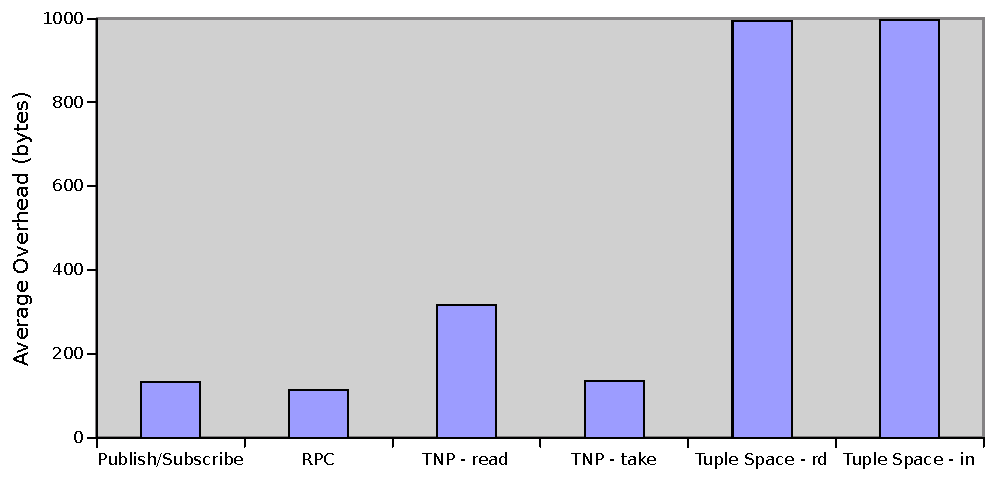
\includegraphics[scale = .70]{overhead.pdf}
\caption{Message Overhead}
\label{fig:overhead}
\end{figure}

AmbientTalk, LIME, and SpatialViews have different methods of providing remote communication. To determine the cost of this communication, we used a simple client-server scenario sending a simple ``hello'' message from the server to a client. The nodes are arranged so that each node is one hope away from any other node.  Figure~\ref{fig:overhead} shows the average message overhead in terms of packets sent per second as the rate of sending messages increases. 

SpatialViews shows the highest amount of overhead, which is expected since it is migrating code and variables to communicate a simple message. LIME requires some communication to alert merged tuple spaces of the messages' presence and then more communication to actually transfer the tuple. AmbientTalk has the lowest overhead, as it is simply performing a method call on a remote object and there is no return value.

\subsection{Multicast Performance}

Group communication is common in MANETs, so it is desirable to know how efficiently each project performs multicast communication. In this scenario, there is a single sender communicating with multiple receivers. Each receiver will echo messages back to the sender and the round trip time is measured upon receiving this response. Again, each node is one hop away from all the others, so there is no multihop communication involved.

\begin{comment}
Surprisingly, this graph is the opposite of Figure~\ref{fig:overhead}. Although SpatialViews had the highest message overhead, it is able to send and receive messages considerably faster than LIME and AmbientTalk. AmbientTalk is the slowest although it has the lowest overhead, and LIME remains in the middle. This is likely due to their implementations, as SpatialViews uses a virtual machine written mostly in C, while AmbientTalk is currently implemented as an interpreter in Java. LIME is simply a Java library, so it performs fairly well but slower than SpatialViews as LIME is running on the full Java virtual machine.
\end{comment}


\section{Related Projects}

The following projects have been included for completeness and because they exhibit unique features, but were excluded from the main discussion.

JANE\cite{jane} works by providing an event-based model with guaranteed network feedback. There are no connections which are maintained, but the application will be alerted if an event cannot be delivered. JANE also provides mobility and network emulation software which allows programs to be tested on simulated devices as well as real devices.

Pervaho\cite{pervaho} is another publish/subscribe middleware for MANETs, but includes the concept of persistent publications. This provides the temporal decoupling missing from STEAM.

TypeCast\cite{typecast} is a recent project which uses types to provide efficient routing for messages in a MANET. The type of an object provides addressing and routing information. TypeCast also supports type hierarchies with subtyping and type composition.

EgoSpaces\cite{EgoSpaces} is another tuple space middleware which focuses on context awareness.
\section{Conclusions}

This paper has discussed four challenges specific to mobile ad hoc applications: handling of frequent disconnections, decentralized addressing and discovery, group and one-to-one communication, and context awareness. We then presented and evaluated existing projects based on tuple spaces, remote object handles, event handling, publish/subscribe, and code migration. Finally, two applications were developed using three selected projects in order to evaluate their advantages and disadvantages with actual applications.

Many of the projects discussed here explore how to extend familiar parallel and distributed programming concepts into the MANET environment. While this works to a certain degree, MANETs present a new application environment which requires new programming abstractions, particularly to deal with frequent disconnections and dynamic topologies. Ideally, these abstractions would make the task of developing new applications natural and simpler, without the programmer needing to worry about low-level MANET issues.

The likelihood of a large number of nearby mobile devices supporting the formation of ad hoc networks is growing. Even entertainment devices such as the Nintendo DS and the Microsoft Zune support spontaneous networking when another device is nearby. Applications for MANETs are currently an expanding field and providing the proper abstractions and tools for rapidly developing and testing these applications can make such applications even more common.

\bibliographystyle{unsrt}
\bibliography{refs}
\end{document}
